\documentclass[11pt,a4paper]{article}
\usepackage{amsmath}
\usepackage{amsfonts}
\usepackage{amssymb}
\usepackage{graphicx}
\graphicspath{{Graphics/}} %Setting the graphicspath
\usepackage[utf8]{inputenc}
\usepackage[english]{babel}
\usepackage{lmodern}
% caption einr�cken
\usepackage{caption}
\captionsetup{singlelinecheck=false,
	font=small,
	labelfont=bf,
	format=hang,
}
% Operators
\DeclareMathOperator*{\argmin}{argmin}
\DeclareMathOperator*{\argmax}{argmax}

\author{Sebastian Knigge}
\begin{document}

\section{Discussed models}

This section will introduce the reader into the two Topic modeling approaches which will be compared in this Thesis. The aim of both procedures is to assign one or more topics to different documents. Even if the vocabulary and the notation are similar for both approaches, the notation should be resumed at the beginning of the description of the respective model. The basic structural notation of the data consists of the following variables.\\
A collection of documents is called corpus $D=(\textbf{w}_1,\dots , \textbf{w}_M)$. It consists out of M documents $\textbf{w}=(w_1,\dots, w_N)$ which are itself separated in words $w_i$. These words are vectors of length $V$. $V$ refers to the length of a vocabulary which holds all the words occurring in the corpus. The vector for a specific word $w_i$ contains all 0 except for index $j\in\{1,...,V\}$ which represents this very one word in the vocabulary.\\
This notation may indeed be extended through the addition of indices for documents, but this is not done here or in the standard literature on topic models due to its unnecessary complexity.\\

\subsection{LDA model}

Latent Dirichlet Allocation is a Bayesian approach and is often associated with the class of hierarchical models \cite{Gelman2014}. The idea is based on the representation of exchangeable random variables (acc. to de Finetti) as mixture of distributions. Given that documents $\textbf{w}$ and words $w_i$ in each document - both considered as random variables in this setting - are exchangeable in such a way, a mixed model such as the LDA model is appropriate.\footnote{Cf. \cite{Blei2003}}\\

The following notation is used in conjunction with the LDA model. Let $z_j$ be the topics with $j\in\{1,\dots,k\}$. In the LDA setting we assume for  every topic $z_j$ there is a term distribution
$$\beta_j \sim Dir(\delta)$$
We further assume each document w has a distribution of topics.
$$\theta \sim Dir(\alpha)$$
Then each word $w_i$ of $\textbf{w}$ is generated by the following process:

\begin{enumerate}
	\item Choose $z_i \sim Mult(\theta)$
	
	\item Choose $w_i \sim Mult(\beta_i)$ This distribution will be referred to as $p(w_i|z_i,\beta)$
\end{enumerate}
\ \\
You can summarize this setup in a plate diagram as shown in figure \ref{fig:PlateDiagram}. The notation above, which is also used within the diagram, coincides with the notation of \cite{Hornik2011}.\\


\begin{figure}[h]
	\centering
	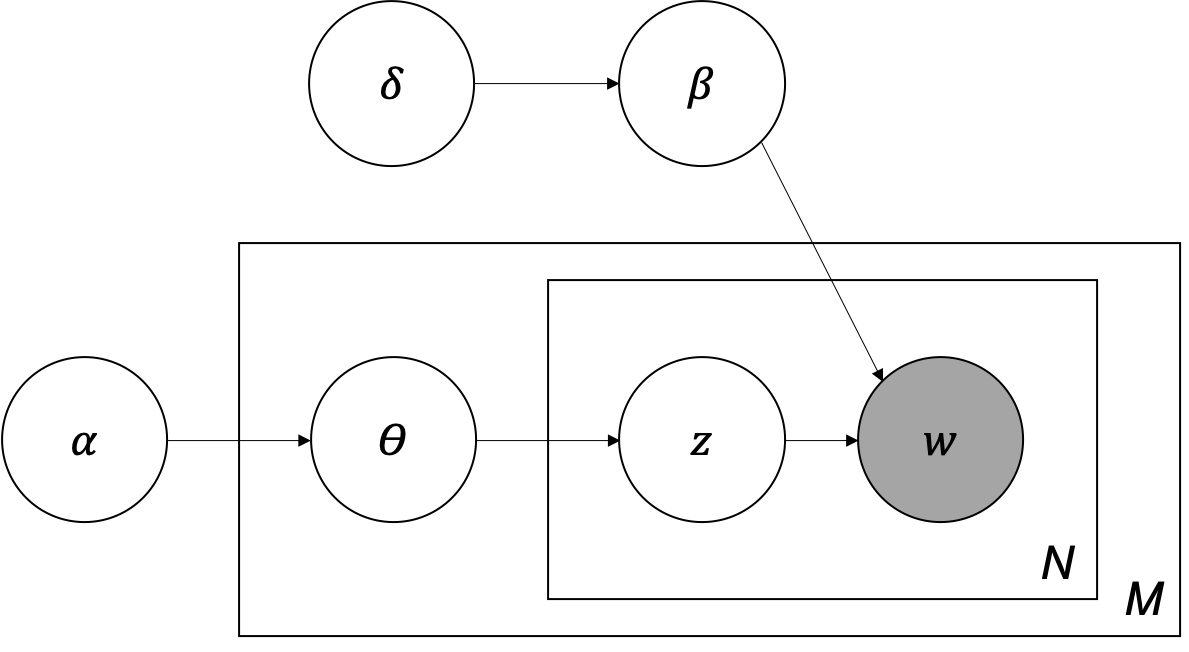
\includegraphics[width=0.5\textwidth]{LDA_Plate_Diagram.png}
	\caption{The well-established plate diagram for the standard LDA model extended by the parameter $\delta$. The slightly bigger box represents the generative model of the corporis $M$ documents. The smaller plate represents the iterative generation process of the $N$ words of each document with the aid of the topics. See also "smoothed LDA model" in \cite{Blei2003}  for comparisons.}
	\label{fig:PlateDiagram}
\end{figure}

In order to estimate the model parameters, the first task is to calculate the posterior distribution, which consists of the joint distribution in the numerator and the marginal distribution in the denominator.

\begin{align}\label{posterior}
	p(\theta,\textbf{z}|\textbf{w},\alpha,\beta)= \frac{p(\theta,\textbf{z},\textbf{w}|\alpha,\beta)}
	{p(\textbf{w}|\alpha, \beta)}
\end{align}
The joint distribution numerator can be derived straight forward.

\begin{align}\label{joint}
	p(\theta,\textbf{z},\textbf{w}|\alpha,\beta)=p(\theta|\alpha)\prod_{i=1}^{N}p(w_i|z_i,\beta)\ p(z_i|\theta)
\end{align}
One can obtain the marginal distribution of a document $\textbf{w}$, by integrating out the parameter $\theta$ and summing over the topics $z_j$. Nevertheless, this expression is intractable.
\begin{align}\label{marginal}
p(\textbf{w}|\alpha, \beta)=\int p(\theta|\alpha) \left( \prod_{i=1}^{N} \sum_{z_i}p(z_i|\theta)p(w_n|z_i,\beta) \right) d\theta
\end{align}
\ \\
According to the current state of research, there are two feasible approaches to calculating the posterior density.\footnote{Cf. eg. \cite{Blei2012}} One approach is to simulate the posterior density by iteratively sampling - the so-called Gibbs sampling. The second approach is a deterministic method, a modified version of the well-known EM algorithm \cite{Dempster1977}: the Variational EM algorithm (VEM algorithm) \cite{Wainwright2008}. In the following two sections the both approaches are roughly outlined to give the reader some insight into the Bayesian inference underlying the algorithms.

\subsubsection{Variational EM algorithm}

In the VEM algorithm for the LDA model is a mean field approach which varies the steps E and M of the EM algorithm in a way such that this algorithm becomes solvable. Note that the main problem of calculating the marginal distribution is, to derive the conditional probability of some hidden variables given some observed values ("evidence"). The variation of the EM algorithms consists mainly in approximating the directly intractable E step.  Rewriting the log of the border density of $\textbf{w}$ as follows in (\ref{marginal2}), results in the fact that the marginal density can be estimated downwards with the aid of Jensen's inequality.
\begin{align}\label{marginal2}
	\log p(\textbf{w}|\alpha, \beta) &= \log \int \sum_{z} 
	p(\theta,\textbf{z},\textbf{w}|\alpha,\beta)d\theta\\
	& =\log \int \sum_{z} \frac{p(\theta,\textbf{z},\textbf{w}|\alpha,\beta) q(\theta,\textbf{z})}{q(\theta,\textbf{z})}d\theta\\
	&\geq \int \sum_{z} q(\theta,\textbf{z})\log p(\theta,\textbf{z},\textbf{w}|\alpha,\beta) d\theta - 
	\int \sum_{z} q(\theta,\textbf{z})\log q(\theta,\textbf{z})d\theta\\
	&= \mathbb{E}_q[\log p(\theta,\textbf{z},\textbf{w}|\alpha,\beta) ]-
	\mathbb{E}_q[\log q(\theta,\textbf{z})] \label{KL}
\end{align}
Here $q(\theta,\textbf{z})$ is an arbitrary distribution which can be called the variational distribution. 
\begin{align}
q(\theta,\textbf{z})\widehat{=}q(\theta,\textbf{z}|\gamma,\phi)
=q(\theta|\gamma) \prod_{i=1}^N q(z_i|\phi_i)
\end{align}
The right hand side $L(\gamma,\phi,\alpha, \beta):=\mathbb{E}_q[\log p(\theta,\textbf{z},\textbf{w}|\alpha,\beta) ]-
\mathbb{E}_q[\log q(\theta,\textbf{z})]$ be called "lower bound". It can be shown that $\log p(\textbf{w}|\alpha, \beta) - L(\gamma,\phi,\alpha, \beta)$ is the Kullbak Leibler divergence ($D_{KL}$) of the true posterior and the variational distribution. From equations (\ref{marginal2})-(\ref{KL}) follows that:
\begin{align}\label{equality}
\log p(\textbf{w}|\alpha, \beta)= D_{KL}(q(\theta,\textbf{z}|\gamma,\phi)||p(\theta,\textbf{z},\textbf{w}|\alpha,\beta)) + L(\gamma,\phi,\alpha, \beta)
\end{align}
Since the marginal is fixed, we conclude, that minimizing the KL-divergence is equivalent to maximizing the lower bound.\footnote{See \cite{Jordan1999} and \cite{Wainwright2008}, for details of the derivation of the lower bound see \cite{Blei2003}}
\begin{align}
(\gamma^*, \phi^*) &= \argmin_{\gamma, \phi}D_{KL}(q(\theta,\textbf{z}|\gamma,\phi)||p(\theta,\textbf{z},\textbf{w}|\alpha,\beta))\\
&= \argmax_{\gamma, \phi} L(\gamma,\phi,\alpha, \beta)
\end{align}\\

The variation of the EM algorithm thus is to use the variational distribution $q(\theta,\textbf{z}|\gamma^*(\textbf{w}), \phi^*(\textbf{w}))$ instead the posterior distribution $p(\theta,\textbf{z},\textbf{w}|\alpha,\beta)$. Now the two steps of the VEM algorithm are:
\begin{itemize}
	\item [(1)]\textbf{E step} Optimize the variational parameters $\theta$ and $\phi$ for every document in the corpus. This can be done analytically by deriving the derivatives of the KL divergence. And set them to zero.
	\item [(2)] \textbf{M Step} Maximize the lower bound using the optimized parameter of the E step with respect to $\alpha$ and $\beta$.
\end{itemize}


\subsubsection{Gibbs sampling}

The second method to approximate the posterior distribution is Gibbs sampling, a so-called monte Carlo method. Instead of calculating the distributions for $\beta$ and $\theta$, the primary task is to find the posterior distribution over $\textbf{z}$ given the document $\textbf{w}$. Gibbs sampling is also known as a Markov Chain Monte Carlo method. The name refers to the simulation process by which a chain of values is simulated whose limiting distribution desirably converges against the true distribution. (\ref{Gibbs}) shows the distribution, which is sampled from iteratively.\footnote{Cf. \cite{Griffiths2006}}
\begin{align}\label{Gibbs}
	p(z_i=j|z_{-i},w)\propto \frac{n_{-i,j}^{(l)}+\delta}{\sum_t n_{-i,j}^{(t)}+V\delta}
	\frac{n_{-i,j}^{(d_i)+\alpha}}{n_{-i}^{(d_i)}+k\alpha}
\end{align}
	\makebox[1cm][l]{$z_{i}=j$} 		... \makebox[5cm][l]{word-topic assignment of word $i$ to topic $j$}\\
	\makebox[1cm][l]{$z_{-i}$}   		... \makebox[4cm][l]{vector of word-topic assignments without the entry for word $i$}\\
	\makebox[1cm][l]{$n_{-i,j}^{(l)}$}	... \makebox[4cm][l]{number of times the $l$th word in the vocabulary is assigned to }\\
	\makebox[1cm][l]{}						\makebox[4cm][l]{\ \ \ \ topic $j$, not including the assignment for word $i$}\\
	\makebox[1cm][l]{$d_i$}				... \makebox[4cm][l]{document in the corpus which includes word $i$}\\
	\makebox[1cm][l]{$\delta,\alpha$} 	... \makebox[4cm][l]{parameters of the prior distributions for $\beta$ and $\theta$}\\

Usually the word-topic distributions $\beta_{j}^{(l)}$ for the words $l=1,...,V$ and topics $j=1,..,k$ and topic-document distributions $\theta_j^{(d)}$ for the documents $d=1,...,D$ and the topics $j=1,...,k$ will be of interest. (\ref{Gibbs:beta}) and (\ref{Gibbs:theta}) shows the predictive distributions denoted as "estimators".\footnote{For derivation and more details regarding the Gibbs sampling procedure see \cite{Griffiths2006}}
\begin{align}
	\hat\beta_{j}^{(l)}&=\frac{n_{-i,j}^{(l)}+\delta}{\sum_t n_{-i,j}^{(t)}+V\delta} \label{Gibbs:beta} \\
	\hat\theta_j^{(d)}&= \frac{n_{-i,j}^{(d_i)+\alpha}}{n_{-i}^{(d_i)}+k\alpha} \label{Gibbs:theta}
\end{align}

\subsubsection{Implementation}

In this thesis, the implementation of the LDA model and its estimation is mainly based on using the package \textit{topicmodels}\footnote{See \cite{Hornik2011}} of Kurt Hornik. The package \textit{topicmodels} can apply both the VEM algorithm as well as Gibbs sampling in order to fit the model. In addition, the package \textit{tidytext}\footnote{See \cite{Silge2017}} is being used for text structuring and embedding. Whereby there are other packages besides this implementation of the LDA model, topicmodels is particularly convenient, because tidytext was designed by its developers to work perfectly in combination with topicmodels.









	
  \bibliographystyle{apalike}
  \bibliography{MagLibrary}

	
	
\end{document}